\documentclass[]{article}
\usepackage[draft]{fixme}
\usepackage{url}
\usepackage[pdftex]{graphicx}


\title{Implementing the Overture Automatic Proof System for VDM}

\author{Miguel Alexandre Ferreira\\
        Software Improvement Group\\
		The Netherlands\\ 
		\texttt{m.ferreira@sig.nl}}

\date{\today}

\begin{document}

\maketitle
\begin{abstract}
This paper reports on the implementation of the Overture Automatic Proof System as a tool-chain of components.
Each component borrows specific functionalities to the tool-chain, enabling the system to discharge VDM proof obligations with the theorem prover HOL.

In previous research work, Sander Vermolen has produced a formal model of a VDM to HOL translator, together with HOL tactics that allow VDM proof obligations to be automatically discharged in the theorem prover HOL.
%Vermolen's prototype is complete enough to discharge proof obligations arising from functional VDM++ models.
%However the prototype's performance is very limited as it can only be executed within a VDM++ interpreter.
Through the VDM++ to Java code generator feature provided by the VDMTools, the model was automatically implemented in Java, allowing for its integration in the Overture Automatic Proof System.

The Automatic Proof System is a Java program that promotes the interoperation between a VDM proof obligation generation tool, the VDM to HOL translator, and the theorem prover HOL.
The current paper reports on the challenges and achievements of the Automatic Proof System's implementation, as part of the Overture Tool framework.
\end{abstract}

\section{Introduction}
\label{sec:introduction}

The Overture initiative is a platform that enables researchers, students and practitioners to experiment with software modelling languages and tools~\cite{LarsenBFL08}.
Although the initiative has mainly focused on VDM, due to its open source nature everyone is welcome to contribute with tools and extensions to other languages.
Through Overture, extensions to the different VDM dialects and supporting tools have been proposed, analysed, tested and finally transferred to industrial settings, namely to the VDMTools~\cite{DBLP:journals/sigplan/FitzgeraldLS08}.
The tool that connects VDM to UML~\cite{Lausdahl08,Lausdahl09} is an example of such knowledge transfer industry.
However, Overture's contribution has gone further than that, as new tools have been developed that supersede the functionality provided by the VDMTools.

One of the tools that adds to the capabilities of the VDMTools is the Automatic Proof Support (APS), which is able to discharge proof obligations (POs) arising from functional VDM models, using the theorem prover HOL~\cite{DBLP:conf/tphol/Gordon91}.
Due to VDM's formal semantics it is possible to analyse a VDM model and pinpoint the locations where inconsistencies might occur.
Such inconsistencies can arise from type invariant violations, miss usage of partial functions and mappings, etc.
Furthermore, besides pinpointing possible inconsistencies, it is also possible to generate verification conditions that if proven to be true assure the model's consistency.
In a VDM context, these verification conditions are deemed POs.

\begin{figure}
  \begin{center}
    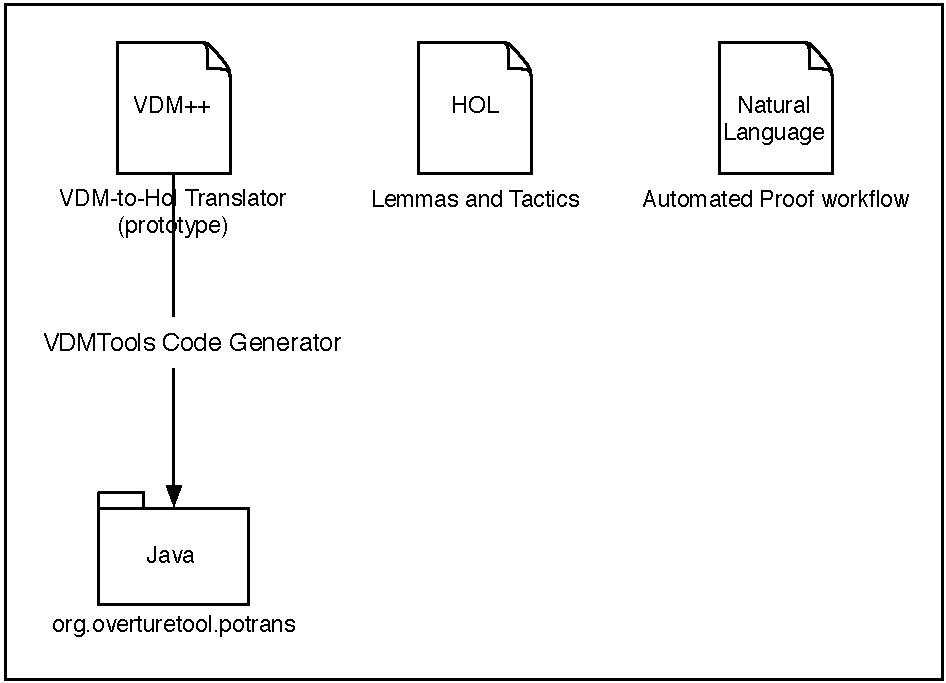
\includegraphics[width=.6\textwidth]{images/vermolen_contribution.pdf}
    \caption[Vermolen's contribution]{Deliverables from Sander Vermolen's MSc project.}
    \label{fig:sander_deliverables}
  \end{center}
\end{figure}

The APS was designed by Sander Vermolen during his MSc project~\cite{Vermolen07}.
The deliverables from Vermolen project, as depicted in Figure~\ref{fig:sander_deliverables}, are:
\begin{itemize}
  \item a VDM++ formal model of a prototype tool that translates VDM to HOL (the Overture VDM-to-HOL Translator);
  \item a Java implementation of the prototype that was automatically generated using the VDMTools;
  \item a set of lemmas which he identified as useful in a VDM context;
  \item and a set of HOL tactics to automate the proofs.
\end{itemize}

The contribution described in this paper focused on the development of the core of the APS , and the integration of several external components.
The external components are integrated through Java interfaces, allowing for a loose coupling between them and the APS core.
Furthermore, the external components were wrapped in utility classes that handle their intrinsic specificities, and were plugged into the APS by implementing the appropriate interfaces.
Figure~\ref{fig:aps_contrib} depicts an abstraction of the APS tool-chain, from which the core, wrapper and utility classes, and their integration are the main contributions from this paper.
Note that the external components inside the wrappers were previously available.

\begin{figure}
  \begin{center}
    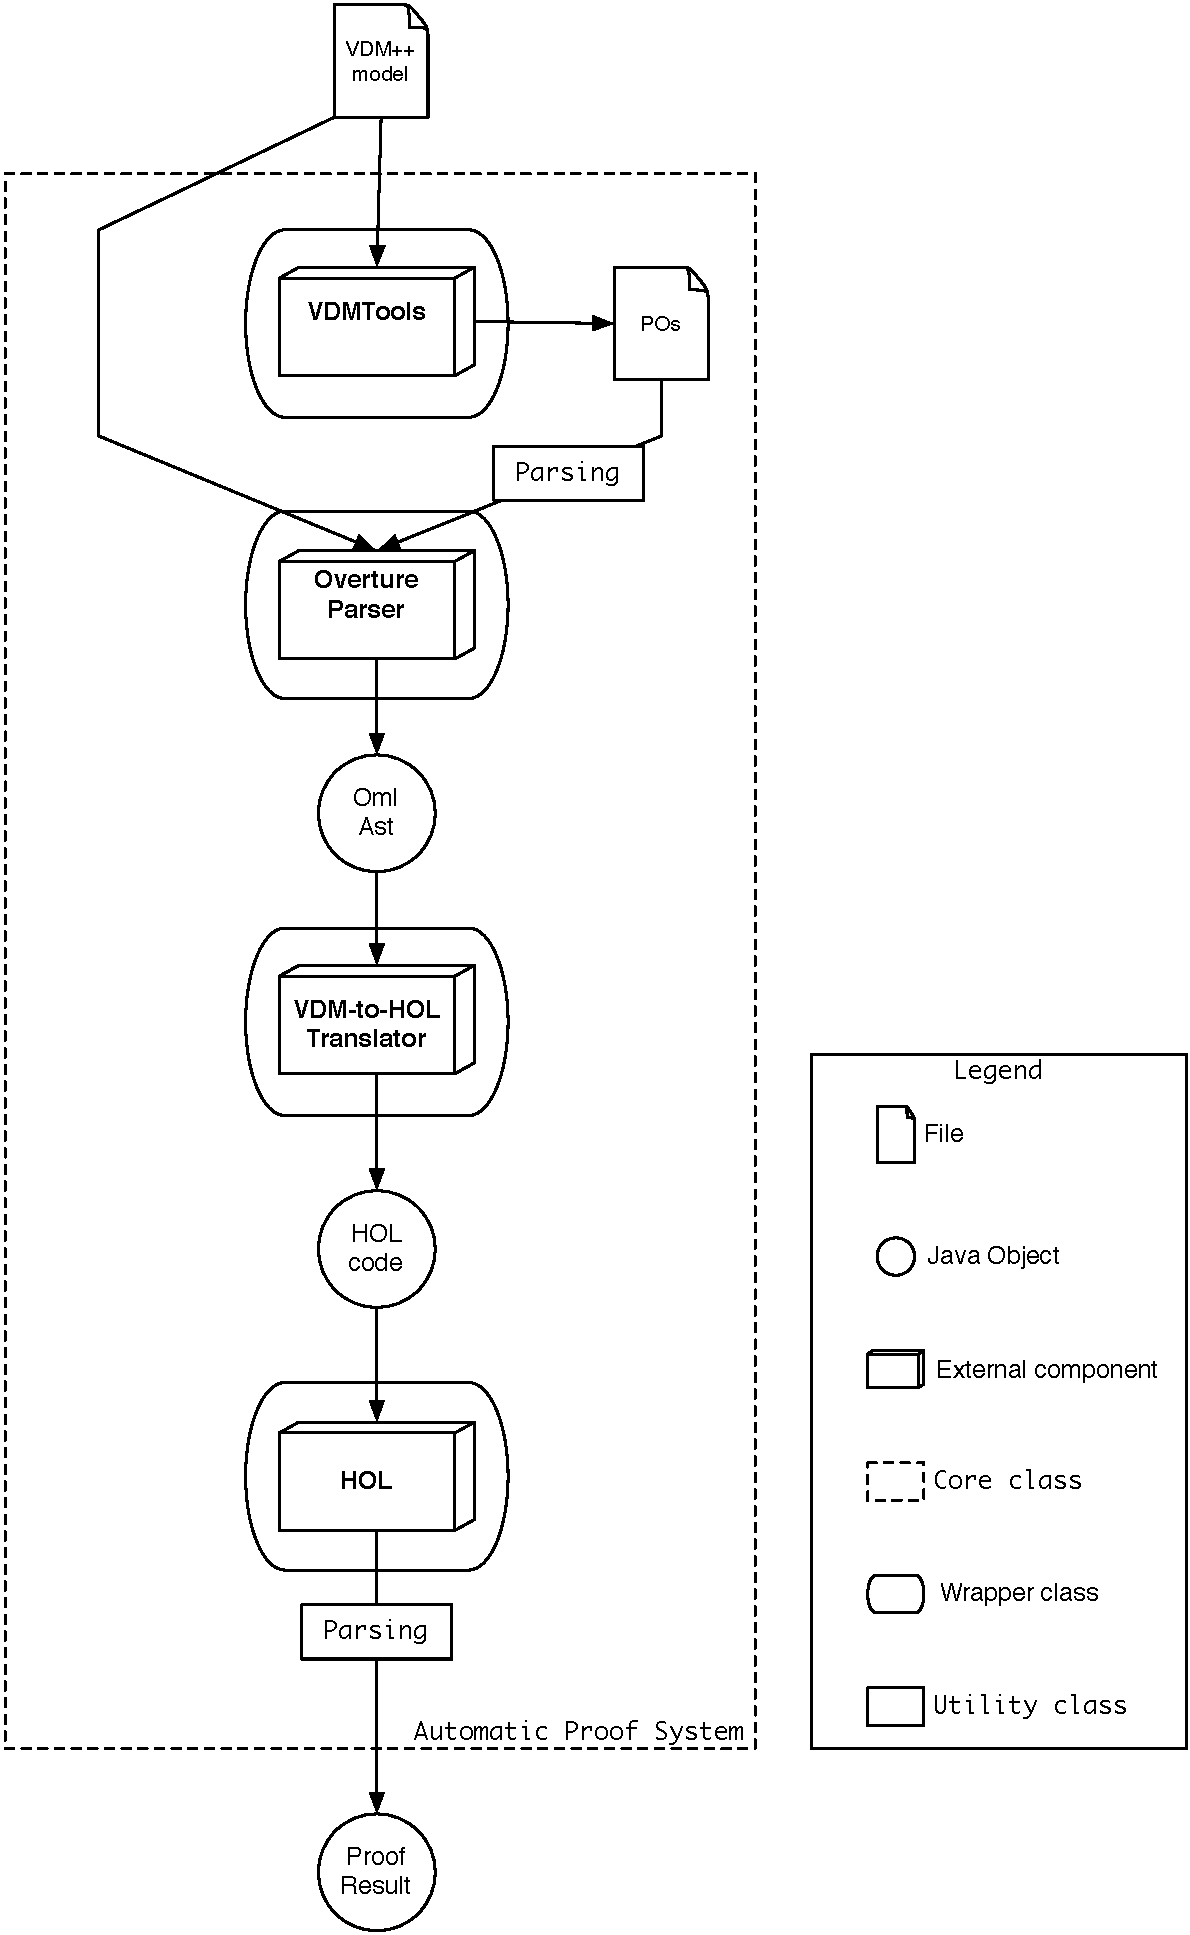
\includegraphics[width=.6\textwidth]{images/tool_chain.pdf}
    \caption[APS tool-chain]{The Automated Proof System tool-chain.}
    \label{fig:aps_contrib}
  \end{center}
\end{figure}


In the next section Vermolen's architecture for APS is described together with the discussion of the difficulties to implement it, and possible solutions.
Section~\ref{sec:implementation} covers the actual implementation issues both at architectural and implementation level.
Future work is presented in Section~\ref{sec:future_work}, and the paper terminates with some conclusions in Section~\ref{sec:conclusion}.



\section{Design}
\label{sec:intended_design}

%Sander's architecture \ldots
%Description of components \ldots
%
%Automated proof achieved in three steps: preparation, translation, proof.
%
%Preparation:
%- convert model's concrete syntax in abstract syntax
%- generate POs from model's AST. POs are already in AST format
%Translation:
%- VDM AST to HOL AST (model + POs)
%- combine HOL AST model with HOL AST POs
%Proof:
%- HOL code generation
%- HOL tactics selection

The APS workflow as originally designed by Vermolen divides the system's operation in three sequential steps, as depicted in Figure~\ref{fig:sander_arch}: preparation, translation, and proof.

\begin{description}
  \item[Preparation.] Preparation is the step that converts a VDM model concrete syntax into the abstract syntax tree (AST) format, as expected by the translator tool.
	It's also in the preparation step that the POs, arising from the model, get generated by a PO generation (POG) tool.
	The POG performs an analysis of the model's abstract representation and produces the PO expressions in the same abstract format (Figure~\ref{fig:arch_preparation}).

  \item[Translation.] Given both model and POs abstract representation, in the translation step, an abstract representation of an equivalent HOL model is created. 
	The translated HOL model consists of a theory, obtained from the VDM model, and a set of proof commands, obtained from the VDM model's POs (Figure~\ref{fig:arch_translation}).

  \item[Proof.] In last step of§ the workflow, the proof, the concrete HOL syntax is generated from its abstract representation and a proof tactic is selected for each PO, according to its type~\footnote{There are several types of PO. For more detailed information see~\cite{CSK:2007lr}}. The last activity in the workflow is the actual proof carried out in the theorem prover (Figure~\ref{fig:arch_proof}).
\end{description}

Following from the described workflow, the architecture of the system is composed of three high level components, one per each step.
Each of these high level components can be decomposed in sub components, which may be part of the APS itself, or external tools that need to be integrated.

\begin{figure}
  \begin{center}
    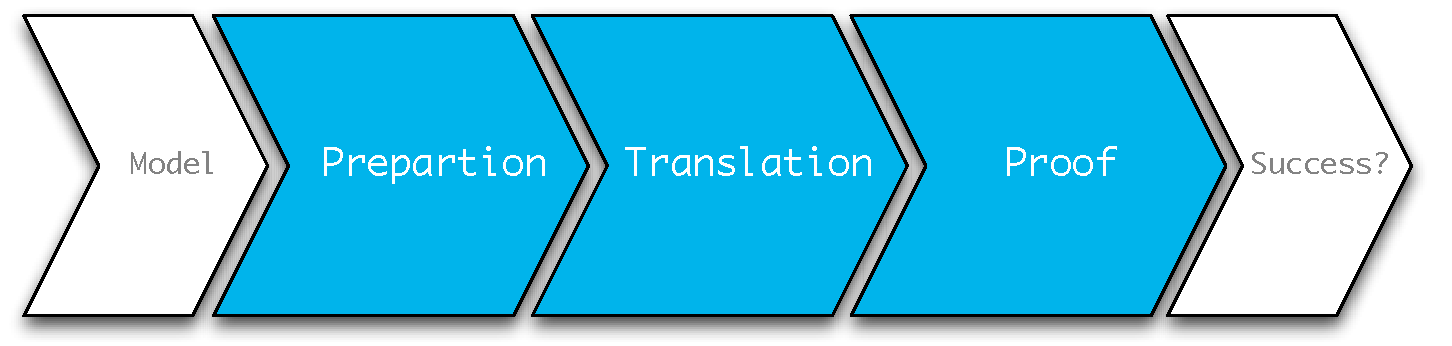
\includegraphics[width=.6\textwidth]{images/pic_arch.pdf}
    \caption[APS workflow]{Automatic Proof System workflow as designed by Sander Vermolen.}
    \label{fig:sander_arch}
  \end{center}
\end{figure}

\begin{figure}
  \begin{center}
  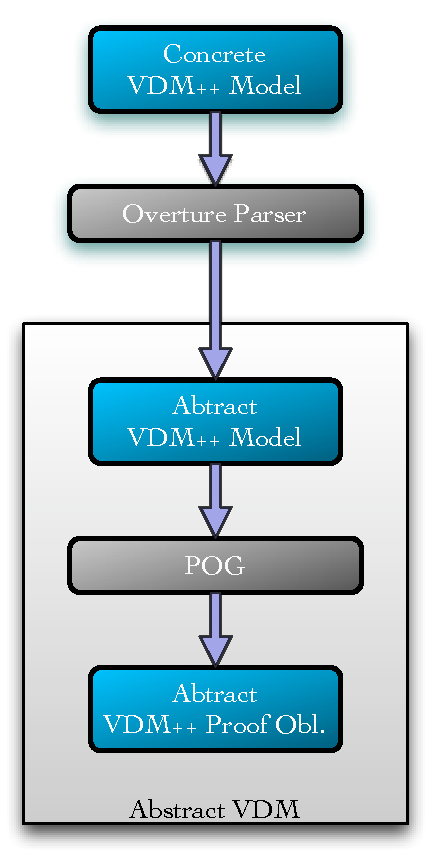
\includegraphics[height=.28\textheight]{images/pic_preparation.pdf}
  \caption[Preparation workflow]{Preparation step workflow as designed by Sander Vermolen. (Diagram obtained from~\cite{Vermolen07}.)}
  \label{fig:arch_preparation}
  \end{center}
\end{figure}

\begin{figure}
  \begin{center}
  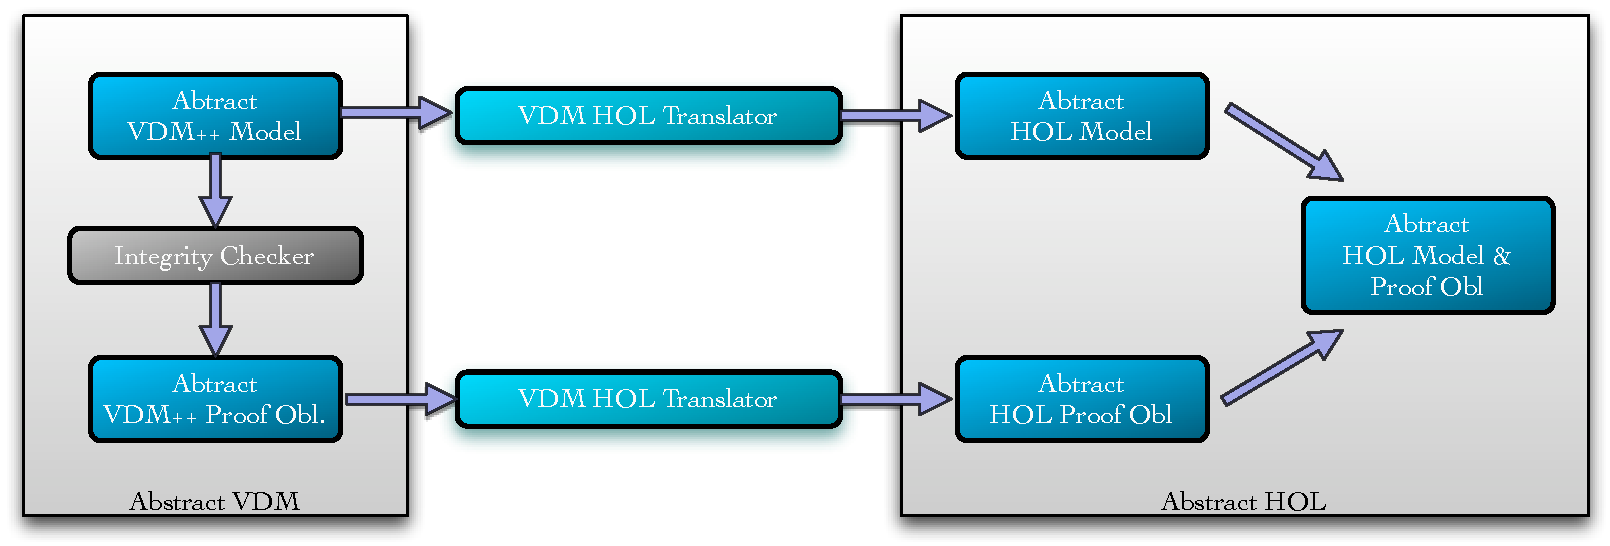
\includegraphics[width=.65\textwidth]{images/pic_translation.pdf}
  \caption[Translation workflow]{Translation step workflow as designed by Sander Vermolen. (Diagram obtained from~\cite{Vermolen07}.)}
  \label{fig:arch_translation}
  \end{center}
\end{figure}

\begin{figure}
  \begin{center}
  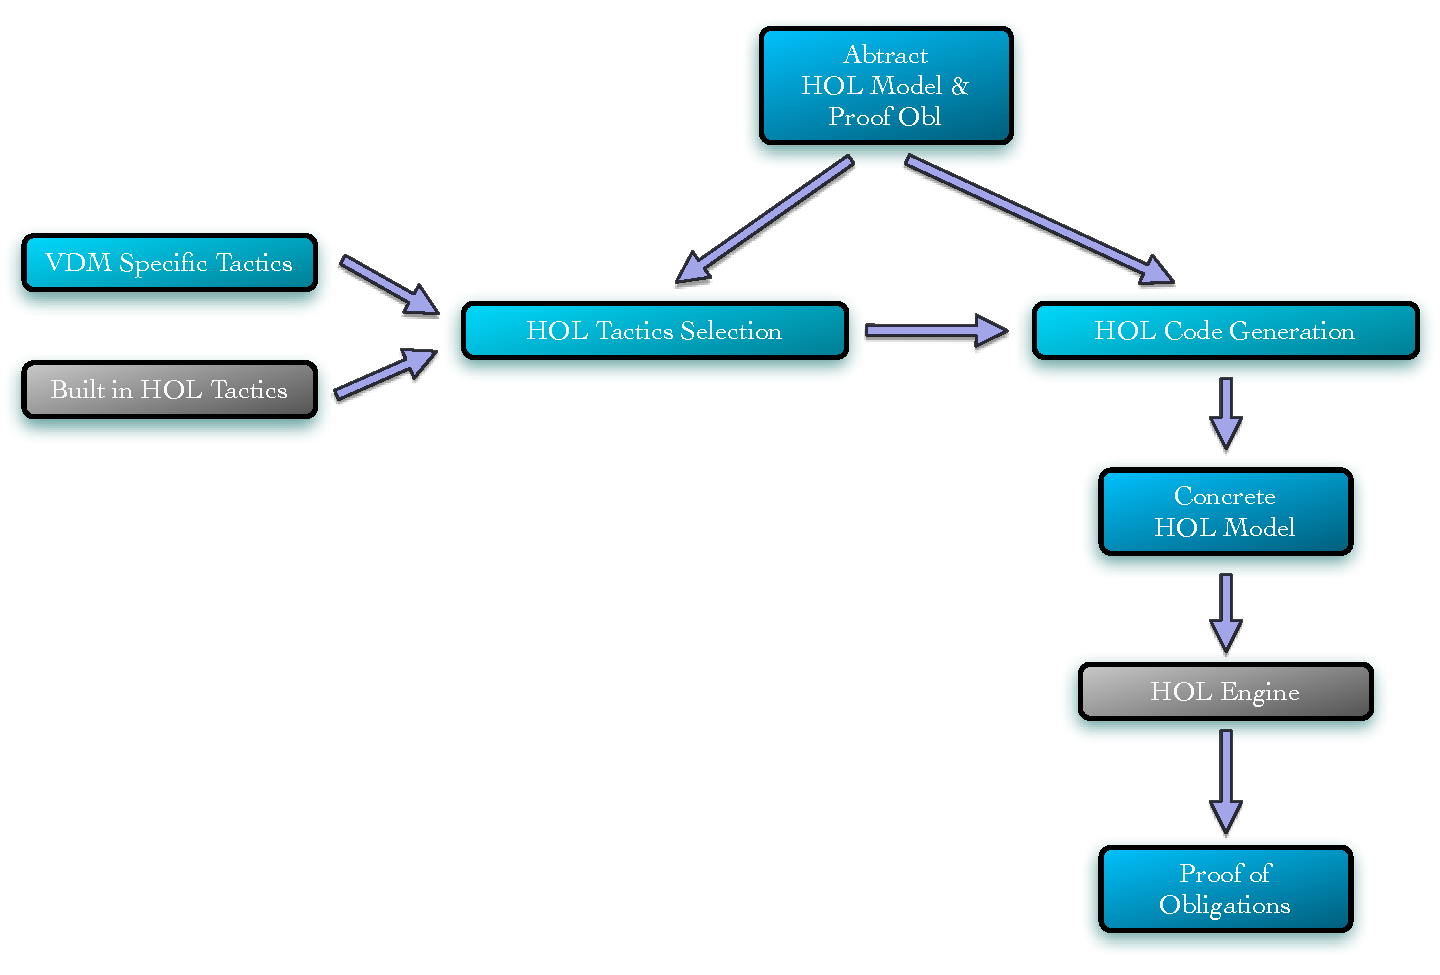
\includegraphics[width=.65\textwidth]{images/pic_proof.pdf}
  \caption[Proof workflow]{Proof step workflow as designed by Sander Vermolen. (Diagram obtained from~\cite{Vermolen07}.)}
  \label{fig:arch_proof}
  \end{center}
\end{figure}


\subsection{Adjustments}
\label{sub:adjustments}

The architecture, as described up until now, can be regarded as the ideal architecture for a scenario where all external tools provide the necessary features.
However, this is not yet the case and two adjustments have to be made.

% There is no POG that generates AST \ldots
The first thing to notice is that, although Vermolen's design makes perfect sense, there is no available combination of POG tool and public VDM AST format to be used in preparation (Figure~\ref{fig:arch_preparation}).
His design decision was based on Overture's pretension to have its own POG tool, which hasn't yet happened.

There are two POG tools that can be used, both belonging to tool sets that are implemented in monolithic packages: the commercial VDMTools and the open source VDMJ.
Moreover, the translation tool, in the translation step, expects both the model and POs to be in the Overture Modelling Language (OML) AST representation, and neither of the POG tools available expects the model to be in this format, let alone generating POs in OML AST.
Both POG tools expect the models to be in VDM concrete syntax and produce textual, human readable, representations of the POs.
This mismatch between the available tools and the intended architecture makes it necessary to adjust the architecture by introducing the Overture Parser as part of the preparation step, as depicted in Figure~\ref{fig:aps_class}.
In this arrangement the system uses the Overture Parser to generate OML AST representations for the model and each POs individually.

% The HOL code generation and tactics selection is done by the translator tool
The second adjustment is related with the proof step, more specifically with the HOL concrete syntax generation and tactics selection (Figure~\ref{fig:arch_proof}).
Both of these activities are performed by the translation tool (if seen as a black box), and therefore they are performed in the translation step instead of the proof step.
However, from the experience gathered from using the APS in some case studies~\cite{FerreiraSO2008,Ferreira2009,FerreiraSBMF09}, the tactics selection as done by the translation tool is suboptimal as the same tactic gets chosen for each and every type of PO.
This issue was not yet addressed in the APS and is left as future work (see Section~\ref{sec:future_work}).

\section{Implementation}
\label{sec:implementation}

The APS is a component of the Overture Tool, and therefore must abide by the development standards of the Overture initiative~\cite{LarsenBFL08}.
The Overture Tool is a formal modelling and verification tool suite that is modular, and integrates in the Eclipse platform through several plugins.
The main implementation language is Java and the APS is no exception to that.

Figure~\ref{fig:aps_contrib} clearly shows that the APS is mainly a tool-chain of components that contribute to the system's goal.
All the computations that are in fact implemented in the APS are either to promote interoperation of the components, or to increase usability.

%Integration of components \ldots
As far as the integration of components goes the implementation uses two ways to achieve it:
\begin{itemize}
  \item direct calls from Java code using external component's public APIs;
  \item or through the command line interface (CLI) of external processes.
\end{itemize}

Both Overture Parser and the Overture VDM-to-HOL Translator have publicly available Java APIs and therefore can be seamlessly integrated with the APS.
As for the generation of POs, the VDMTools was chosen to perform the underlying tasks, and because its CORBA interface doesn't provided the necessary API, the interoperation was done through the CLI.
The choice here could have been VDMJ as it offers a Java API that could be called directly from the APS code.
However, VDMJ's POG was still under development at the time of the implementation, and the one from VDMTools is much more mature and heavily.
This doesn't mean that the APS relies exclusively on the VDMTools, because the PO generation and parsing of their textual representations are abstracted by Java interfaces (Figure~\ref{fig:aps_class}), which provide the desired decoupling from implementations.
Although VDMJ is not yet supported as a POG tool for the APS, the system is prepared to allow its integration in the tool-chain (see Section~\ref{sec:future_work} for more information on this subject).
The CLI is also used to interoperate with the theorem prover HOL.

% Interoperation
The interoperation of the different tools though CLI raises some difficulties in terms of parsing the output of a tool to supply the needed data to the next.
This difficulties are due to the nature of CLIs, as these are meant to be operated by humans.
The most notorious example is the parsing of the list of POs generated by the POG component.
If the tool (in this case the VDMTools) would provide a machine readable format, like XML for instance, it would make the implementation a lot simpler and cleaner.
Also the output from HOL must be parsed to check whether the translated HOL code is correct or contain errors, as well as to check the result from a  proof.

Interoperation with the CLI of the different components was implemented through a \emph{console} abstraction layer (Figure~\ref{fig:aps_console_class}).
The \emph{console} mimics the behaviour a human expects from the CLI of a tool, as well as the behaviour the tool expects from its users.
This implementation decision helped clear the clutter involved in the interaction with the CLIs, as well as to better structure and re-utilize code.
On top of the \emph{console} abstraction layer wrapper objects were implemented for each component, taking advantage of methods the layer provides and adding more, component specific, features.
Furthermore all external component wrapper implement a specific interface to interact with the APS core (Figure~\ref{fig:aps_class}).

\begin{figure}
  \begin{center}
    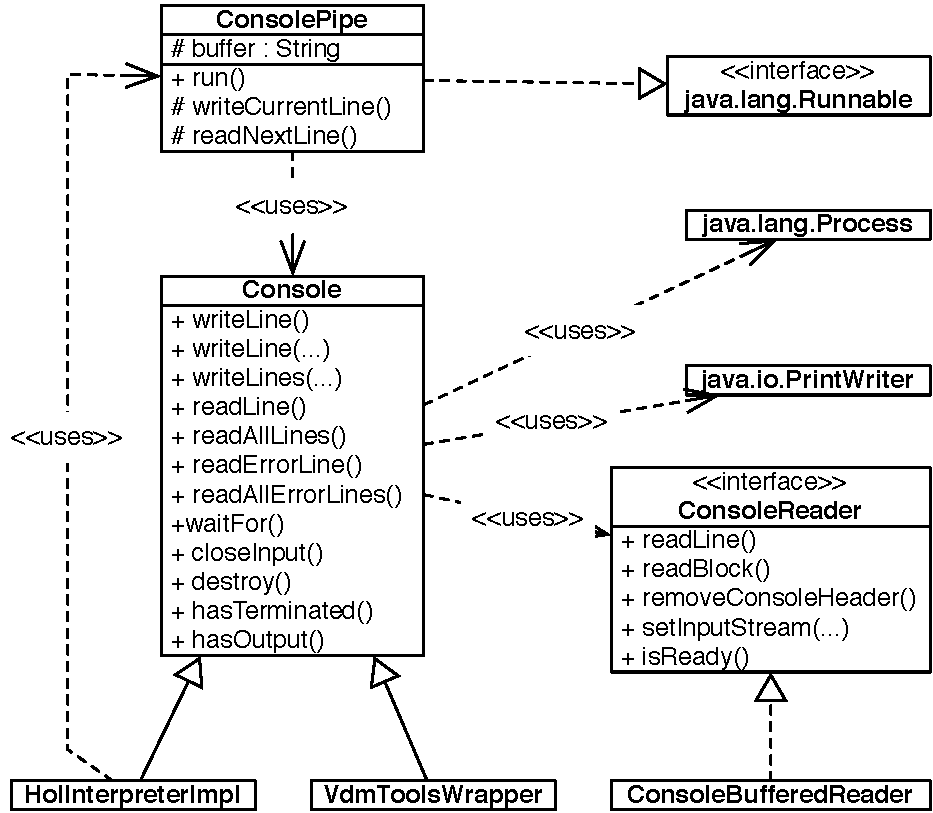
\includegraphics[width=.8\textwidth]{images/aps_console_class_diagram.pdf}
    \caption[Console asbtraction class diagram]{Console abstraction layer class diagram.}
    \label{fig:aps_console_class}
  \end{center}
\end{figure}

%Usability \ldots
Usability issues also arise from the experience obtained using the system as it was still a prototype.
In the one hand, sometimes the VDM specific tactics are not enough to discharge a PO.
On the other hand, sometimes the proof attempts don't terminate in feasible time.
So if the APS was able to detect a failing, or non terminating, proof and allowed the user to try a different tactic, it would increase the success rate of the overall system (see Section~\ref{sec:future_work} for more information).

\begin{figure}%[p]
%  \begin{center}
    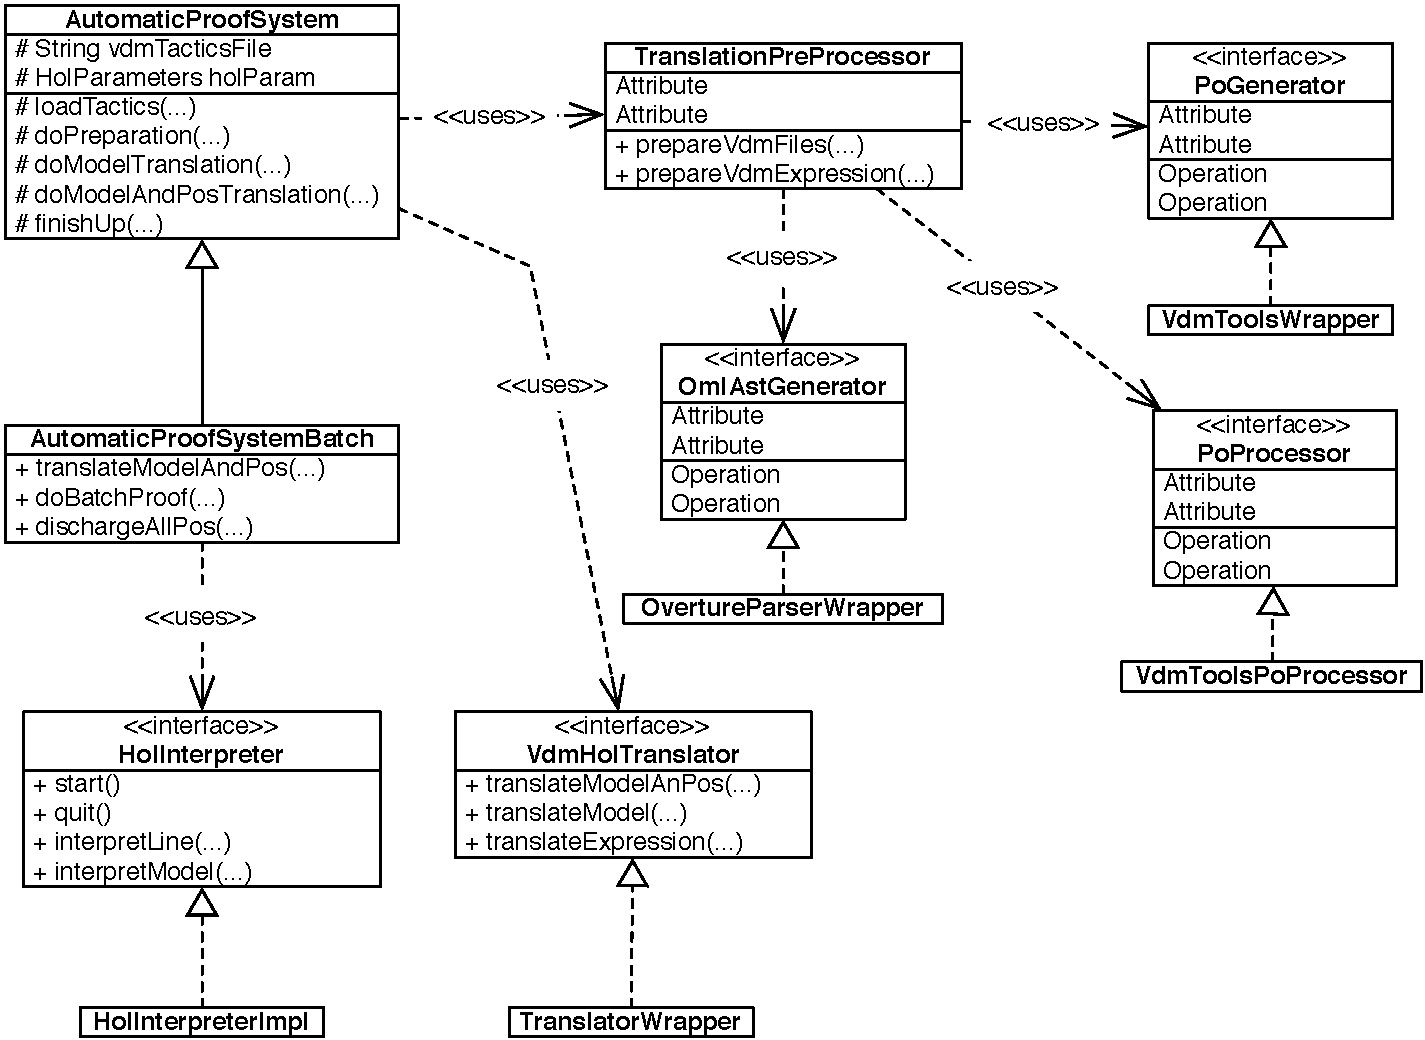
\includegraphics[width=\textwidth]{images/aps_class_diagram.pdf}
    \caption[APS class diagram]{Automatic Proof System class diagram.}
    \label{fig:aps_class}
%  \end{center}
\end{figure}


\subsection{Difficulties}
\label{sub:implementation_difficulties}

% Lack of proper documentation
Documentation, or the lack of it, was one of the major drawbacks during implementation, even regarding components that are part of the Overture initiative.
For instance the Overture Parser has had the capability to parse a single VDM expression separated from the context of a model for a long time now.
This feature is what enables the APS system to generate OML AST representations for each PO individually.
However, during the implementation of the APS the development was stalled for some weeks because there was no knowledge of this feature.
%This lack of knowledge was due to a momentary lack of availability from the implementer of the Overture Parser.
The same goes for the APS, as no documentation whatsoever was created apart from Vermolen's MSc thesis, and this paper.

It is not only on the open source side that documentation lacked. 
The APS uses the VDMTools to generate the POs through the CLI.
However the flag that is used to trigger the PO generation in the VDMTools is also not documented.
Neither in the usage information provided through the CLI, nor the actual manual of the tool.
It was only though the close connection and cooperation with CSK, the current suppliers of the VDMTools, that this information was obtained.

%Java child process bug \ldots
Other major drawback for the implementation of the APS was the way Java handles external processes, and especially child processes\footnote{A child process is a process that is created within another process.} of the processes one instantiates within a Java application.
In a Java application if a process, say $A$, is created and in its turn creates a child process, say $B$, then, if $A$ is terminated and the calling application calls a wait for method on $A$ before $B$ has (somehow) terminated, then the method issued on $A$ will never return.
This means that the wait for method does not return until all child processes are terminated.
However, if a destroy method is called on $A$ it's child processes will not be destroyed, as it is the responsibility of the parent process to terminate its child processes.
This behaviour is well documented in the Java bug/issue tracking system~\footnote{For more details see \url{http://bugs.sun.com/bugdatabase/view_bug.do?bug_id=4770092}.}.

The theorem prover HOL, in its version 4, is built on top of the Moscow ML~\footnote{\url{http://www.itu.dk/~sestoft/mosml.html}} interpreter which an implementation of the Standard ML language interpreter.
This means that HOL runs inside the Moscow ML interpreter.
HOL's executable is in fact a script that pipes its input to a first command, named \emph{unquote}, which basically replaces the quotes in HOL concrete syntax by machine readable markers.
The output of \emph{unquote} is then re-piped to the \emph{ML interpreter}.
So whenever the HOL executable is invoked from the command line two child processes are also invoked, one for \emph{unquote} and another for the \emph{ML interpreter}.
This is the case both in Windows and Unix alike platforms.

It is a good programming practice to wait for the processes to finish.
However, in this case after issuing the HOL process termination command (by supplying it with the proper string), the method that waits for it to finish enters a deadlock state.
On the other hand, if a forced destruction of the HOL process is issued, the result is even worse.
One of HOL's child processes starts to allocate all the memory it could get, until the machine becomea unusable.

To overcome this problem, the implementation never calls HOL's executable directly.
Instead, it creates two independent processes, one for \emph{unquote} and another for the \emph{ML interpreter}.
These two processes are encapsulated using the already mentioned \emph{console} abstraction, and a new thread is created to pipe the output of the first process to the input of the second (Figure~\ref{fig:aps_console_class}).
This way both processes are directly managed by the APS, thus avoiding the unwanted behaviour of Java.

\subsection{Current Status}

The APS is currently in its version 1, and is only available as a command line application.
It uses the Args4j~\footnote{\url{https://args4j.dev.java.net}} library to parse command line parameters and arguments.

Testing was done through the jUnit test framework, and 69 unit tests were created to monitor the APS code.
These unit tests amounting to a code coverage of 78.2\%, covering all major components and their interactions.

There are two execution modes: \emph{translation} that simply translates the VDM model and its POs to HOL syntax; and \emph{proof} that not only translates the model but also attempts to discharge the POs directly in HOL.
The execution of the tool in either mode is done in a batch, meaning that inputs are supplied to the tool and it produces an output.

\section{Future Work}
\label{sec:future_work}

%Integration in Eclipse\ldots
Although the APS is useful as a standalone application, the objective is to have it integrated in the Overture Tool as an Eclipse plugin.
This integration can be done in two steps. 
First through a minimalistic plugin that acts as a ``console'' for the APS, simply showing the user the results from each PO proof attempt.
If all goes right with the first, and minimalistic, plugin then a more sophisticated approach could be taken.
This approach would consist in having a graphical user interface (GUI) for the APS, where POs would be displayed in a table aggregating the information of automated proof attempts.
In the case that some POs are not automatically discharged, the GUI would give the user the opportunity to assist the theorem prover.

%Interactive execution \ldots


%Support for VDMJ as a POG tool \ldots
The generation of the POs is an open issue in the context of Overture since there are two available POG tools, but none works at the AST level.
This fact implicates unnecessary parsing and diminishes the interoperability between components.
The APS doesn't yet support VDMJ as a POG generator, although it is prepared for that, and this is also something to be done in the upcoming releases.

%Use timer to avoid non terminating proofs, and be able to try different tactics if a proof takes too long \ldots
Proofs in HOL might not terminate in feasible time.
Therefore the APS must be equipped with, configurable, timers to detect those situations, and abort the proof if necessary.

% Panellisation
Given the current multi-core trend in computer hardware, the APS could take advantage of multi-core architectures to launch proofs in parallel, and with this improve its performance.

% Improve on translation \ldots
Although the translation of VDM syntax in HOL syntax is the responsibility of other Overture component, this is crucial for the usability of the APS.
At the moment the APS, even if was already integrated in the Overture Tool through Eclipse, wouldn't bring so much value to VDM modellers because of the quite small subset of the language supported by the translator.

There are also problems in the translation that were already identified by Vermolen in his thesis~\cite[Section 7.3]{Vermolen07} but remain unresolved.
Some of these issues result in syntax errors in the produced HOL code.

\section{Conclusion}
\label{sec:conclusion}

The APS is basically a tool-chain of components that when properly interoperated work together to discharge VDM POs.
Its implementation was not always straight forward but it was still successful.

Vermolens effort in the formal specification of the translation tool and design of the workflow of the system had a very positive impact in the actual implementation.
Implementing a system like the APS following carefully laid out guidelines certainly reduces the time and cost, as opposed to having an idea and starting to implement it straight away.
Furthermore, the value of the VDM++ formal prototype transcended the prototype's function in the design phase, as the actual Java code, that is being used by the APS, was automatically generated from it.

In conclusion, the basic functionality as designed and formally prototyped by Sander Vermolen is now implemented, but there is still room for improvement.

\bibliographystyle{plain}
\bibliography{mf}

\end{document}